\documentclass[sigconf]{acmart}
\settopmatter{printacmref=false,authorsperrow=3,printfolios=true}
\setcopyright{none}
\renewcommand\footnotetextcopyrightpermission[1]{}
\pagestyle{plain}
\usepackage{graphicx}
\usepackage{booktabs}
\usepackage{multirow}
\usepackage{enumitem}
\usepackage{array}
\usepackage{tabularx}
\usepackage[section]{placeins}
\usepackage{float}
\usepackage{hyperref}
\hypersetup{hidelinks}
\setlength{\emergencystretch}{2em}
% Column-width floats stay with their discussion instead of queuing
% for a later double-column float page.
\setcounter{topnumber}{2}
\setcounter{bottomnumber}{1}
\setcounter{totalnumber}{3}
\renewcommand{\topfraction}{0.85}
\renewcommand{\bottomfraction}{0.7}
\renewcommand{\textfraction}{0.15}
\renewcommand{\floatpagefraction}{0.75}
\setlength{\textfloatsep}{12pt plus 2pt minus 2pt}
\setlength{\intextsep}{10pt plus 2pt minus 2pt}
\acmDOI{}
\acmISBN{}
\acmYear{2026}
\copyrightyear{2026}
\acmConference[Human-Computer Interaction]
{Term Project: Human-Centered AI System (Final Report)}
{2026}{IUT, OIC, Dhaka, Bangladesh}
\title[Explainable Priority at a Smart Intersection]{Explaining Priority at a Smart Intersection: An Exploratory Evaluation of Fair Pedestrian--Vehicle Signal Control}
% Author names and email addresses preserved from the supplied Report_HCI.pdf.
\author{Alif Hasnain}
\affiliation{
  \institution{Department of Computer Science and Engineering\\Islamic University of Technology (IUT), OIC}
  \city{Dhaka}
  \country{Bangladesh}
}
\email{alifhasnain@iut-dhaka.edu}
\author{Afsana Shehrin}
\affiliation{
  \institution{Department of Computer Science and Engineering\\Islamic University of Technology (IUT), OIC}
  \city{Dhaka}
  \country{Bangladesh}
}
\email{afsanashehrin@iut-dhaka.edu}
\author{Maroof Ahmed}
\affiliation{
  \institution{Department of Computer Science and Engineering\\Islamic University of Technology (IUT), OIC}
  \city{Dhaka}
  \country{Bangladesh}
}
\email{maroofahmed@iut-dhaka.edu}
\author{Kazi Akib Zaoad}
\affiliation{
  \institution{Department of Computer Science and Engineering\\Islamic University of Technology (IUT), OIC}
  \city{Dhaka}
  \country{Bangladesh}
}
\email{akibzaoad@iut-dhaka.edu}
\author{Md Saidur Rahman Sagor}
\affiliation{
  \institution{Department of Computer Science and Engineering\\Islamic University of Technology (IUT), OIC}
  \city{Dhaka}
  \country{Bangladesh}
}
\email{saidurrahman@iut-dhaka.edu}
\author{Hasan Mahmud}
\authornote{Corresponding author.}
\affiliation{
  \institution{SSL, Department of Computer Science and Engineering\\Islamic University of Technology (IUT), OIC}
  \city{Dhaka}
  \country{Bangladesh}
}
\email{hasan@iut-dhaka.edu}
\renewcommand{\shortauthors}{Hasnain et al.}

\newcommand{\mw}{R_{\max}}
\newcolumntype{Y}{>{\raggedright\arraybackslash}X}

\begin{document}
\begin{abstract}
A traffic signal decides who waits, but rarely makes the reason visible.
This project explores how pedestrian--vehicle priority can be made more
transparent through Explainable Fair Priority Bargaining (EFPB), a
controller that combines service utilities, waiting-based weights, an
efficiency filter, and structured decision records. We developed a
research prototype and evaluated its implemented allocation rule against
tuned fixed-time, efficiency-only, and equal-weight bargaining controllers.
The main evidence comprises 520 exploratory SUMO/TraCI runs across nine
nominal and four stress demand conditions, with ten paired seeds per
condition. Vehicles and signals were simulated in SUMO; pedestrian
arrivals and service were represented by a virtual queue. Under nominal
demand, EFPB's recorded person-delay proxy averaged 6.31~s, compared with
6.45~s for efficiency-only control and 8.49~s for fixed time. Fixed time,
however, achieved a lower maximum-wait ratio. Under overload, every
controller exceeded the configured waiting limit, and the equal-weight
baseline exhibited severe starvation. These observations support further
investigation of transparent allocation, rather than a claim of universal
superiority. The report connects the prototype to human-centered design
requirements while documenting measurement and implementation limits.
Explanation comprehension, perceived fairness, and trust remain
unevaluated because no participant study was conducted.
\end{abstract}
\keywords{Human-Centered AI, Explainable AI, Traffic Signal Control,
Pedestrian Priority, Fairness, SUMO, Human--Computer Interaction}
\maketitle
\pagestyle{plain}
\thispagestyle{plain}
\raggedbottom

\section{Introduction}
A person waiting at a crossing sees the signal change but cannot usually
tell why another group received priority. An operator faces a related
problem: a controller may report that it reduced average delay without
showing whose waiting time increased. These are allocation decisions with
human consequences. A useful system should make the trade-off visible
and provide enough evidence for someone to question its decision.

This project investigates Explainable Fair Priority Bargaining (EFPB)
for a four-arm signalized intersection. The intended system represents
pedestrians and vehicles through two virtual mode advocates, gives
additional weight to accumulated waiting, and records the reasoning
behind each selection. The advocates are software abstractions. They do
not assume that individual road users negotiate strategically or assign
a monetary value to their right to cross.

The central difficulty is that a good average can hide an uneven
experience. A policy may move many vehicles quickly while making a
smaller pedestrian queue wait repeatedly. Conversely, a policy that
offers very regular service can spend time on a lightly used approach.
We therefore treat efficiency and protection against long waits as
related but distinct objectives. Neither one, by itself, is a complete
definition of fairness.

The original research plan combined a traffic-control evaluation with
an HCI study of factual and counterfactual explanations. The completed
work is narrower: an executable controller prototype, calibration, and
simulation experiments. This report retains that distinction throughout.
It addresses whether the implemented EFPB rule offers a useful
delay--waiting trade-off under nominal demand, and how that trade-off
changes near capacity. Whether people understand or trust its
explanations appropriately remains a question for subsequent research.

Our contributions are an inspectable implementation of a priority
allocator; a paired comparison with three baselines using 520
SUMO/TraCI runs; and design implications drawn from both the results
and the shortcomings revealed during development. The contribution is
the combination of an allocation mechanism, an explanation-oriented
design, and a carefully bounded evaluation. It is not the invention of
Nash bargaining for traffic signals, nor a completed validation of
pedestrian safety or human experience.

Two questions organize the technical evaluation. First, how does
EFPB compare with the baselines when demand remains within the
nominal range? Second, what breaks down when one or both modes
approach saturation? The explanation-oriented design adds a separate
question: what evidence would an operator need to understand those
outcomes? The simulations address the first two questions; the third
guides the design discussion without being presented as a tested
human-subjects result.

\section{Related Work}
Human-Centered AI places human goals, responsibility, and control
alongside automation. Shneiderman's framework motivates systems whose
operation can be inspected and supervised, rather than judged solely by
an optimization score~\cite{shneiderman2022hcai}. For this project,
that means exposing the allocation policy and its limits as well as the
selected signal phase.

Interaction design provides a complementary perspective. Sharp,
Preece, and Rogers emphasize understanding activities and evaluating
designs with users~\cite{sharp2019interaction}. Cooper et al.'s
goal-directed approach helps distinguish the needs of a pedestrian
seeking a predictable crossing opportunity from those of an operator
investigating a recurring delay~\cite{cooper2014aboutface}. These
perspectives inform our requirements and interface proposal. They do
not substitute for the user research that this project still needs.

Traffic allocation using bargaining is already established. Wang et
al.\ use Nash bargaining to allocate green durations while considering
both pedestrians and vehicles~\cite{wang2023bargaining}. Their work
makes clear that multimodal bargaining itself is not a sufficient
novelty claim. Our intended extension concerns waiting-based priority,
a near-efficiency restriction, and decision records designed to support
explanation. The implemented equal-weight comparator is an internal
baseline; it is not a verified reproduction of Wang et al.'s method.

Bargaining is useful here because it makes the representation of each
mode explicit. Nevertheless, its behavior depends on the utilities,
disagreement point, and feasible alternatives supplied to it. Calling
an objective a bargaining solution does not resolve those modeling
choices. Our comparison therefore concerns the particular rules
implemented in this prototype, and the interpretation of the results
must remain tied to those rules.

The explanation literature also cautions against equating more
information with better understanding. Miller describes explanation
as a selective, often contrastive activity~\cite{miller2019explanation}.
This motivates a short account of the chosen action, followed by an
optional comparison with an alternative. Lee and See argue for
appropriate reliance on automation~\cite{lee2004trust}: a person should
recognize a poor decision as well as a sound one. Accordingly, a future
HCI evaluation should test decision understanding and error detection,
not merely ask whether the interface increases trust.

This distinction also separates an explanation from a persuasive
summary. A statement that a controller served pedestrians because
they had waited longer should be recoverable from the decision
record. A statement that another choice would become preferable
under a changed input should survive a replay of that same rule.
These are technical conditions for an explanation worth evaluating;
they do not establish that its wording is clear to a reader.

The gap addressed here is therefore practical and limited: connecting
a transparent multimodal allocation rule to inspectable evidence about
its behavior. SUMO supplies the microscopic vehicle-simulation
environment~\cite{sumo2018}, while the present project examines the
allocation and reporting layer built around it.

\section{Methodology}
\subsection{Requirement Analysis}
The available materials contain a research plan, implementation, and
experiment reports, but no interview transcripts, survey responses, or
observational records from prospective users. Requirements in this
report are therefore derived from the project brief, relevant design
literature, and analysis of the intended tasks. They should be read as
design hypotheses rather than findings from a completed requirements
study. No thematic or affinity analysis of participant data is claimed.

Table~\ref{tab:requirements} connects each goal to the prototype and
states what the current evidence can support.

\begin{table}[!htbp]
\caption{Requirements--goal traceability. Each row separates the design response from its present evidence.}
\label{tab:requirements}
\small
\renewcommand{\arraystretch}{1.12}
\begin{tabularx}{\columnwidth}{@{}>{\raggedright\arraybackslash}p{.23\columnwidth}Y@{}}
\toprule
Requirement & Design response and present status\\
\midrule
R1: Predictable, non-conflicting service &
Minimum green and explicit transitions. Vehicle yellow/all-red states exist; physical pedestrian clearance is absent.\\
\addlinespace[3pt]
R2: Protection against repeated neglect &
Waiting-dependent weights and a maximum-wait check. Predicted-wait filtering and least-breach fallback exist; overload still breaches the limit.\\
\addlinespace[3pt]
R3: Reasonable total waiting &
Predicted-loss comparison and near-efficiency filtering. Assessed through recorded delay and maximum-wait proxies.\\
\addlinespace[3pt]
R4: Understandable decisions &
Structured records and deterministic text. Code support exists; fidelity and comprehension are not established by the matrix.\\
\addlinespace[3pt]
R5: Alternatives and oversight &
Replay-based comparison and history. Bounded search exists; the participant interface and live override remain unimplemented.\\
\addlinespace[3pt]
R6: Reproducible, auditable results &
Paired seeds, frozen settings, version checks, and stored results. All 520 per-run rows and aggregates were checked; raw trajectories were unavailable.\\
\bottomrule
\end{tabularx}
\end{table}

Three stakeholder perspectives guided the analysis. Pedestrians need
timely service and understandable indications of when crossing is
permitted. Drivers and vehicle passengers need predictable signal
transitions and reasonable delay. Operators and researchers need to
inspect decisions, identify failures, and compare policies without
losing the history behind a result. People with slower walking speeds
are an important stakeholder group, although their crossing behavior
was not represented in the completed SUMO experiments.

We use two provisional personas to make these tasks concrete. A
pedestrian waiting while successive vehicle queues receive service
wants to know whether their wait is being considered. An operator
reviewing an overloaded interval wants to know whether a large delay
comes from demand exceeding capacity, a policy choice, or a faulty
implementation. These are constructed scenarios, not profiles inferred
from interviews.

For the operator, the task sequence is to locate a decision, inspect
the recorded state, compare the selected phase with an alternative,
and determine whether further investigation is needed. This sequence
led to the traceability requirements in Table~\ref{tab:requirements}.
Functional requirements concern allocation, logging, and explanation;
non-functional requirements concern reproducibility, clarity, and
reliable execution.

The requirements are deliberately not collapsed into one success
score. R2 asks whether a mode can be neglected, whereas R3 asks
about aggregate waiting. A controller could satisfy one more closely
than the other. Similarly, R4 requires an account of a decision, while
R5 asks whether that account can be questioned. Keeping these goals
separate makes it possible to report partial progress without treating
a low delay value as proof that all user needs have been met.

\subsection{Design and Prototyping}
The design separates allocation, execution, and explanation. Allocation
chooses a target phase from a small candidate set. Execution applies
the signal state and transition timing. Explanation uses the decision
record to describe the choice. This separation supports R1 and R4:
an understandable recommendation is useful only if the signal
actually executes the intended action.

The prototype was developed with Python, YAML configuration files,
SUMO/TraCI, and structured JSON/CSV output. Its main implemented
interface is a command-line experiment workflow. There is no evidence
of a completed Figma prototype or participant-facing dashboard, so
neither is presented as an evaluated artifact.

For a future explanation interface, the proposed layout places signal
status first, waiting information second, and the rationale below them.
An optional disclosure would explain why another phase was not
selected or show a replay-validated change. This ordering follows the
operator's task: establish what happened before interpreting why.
History and data-age indicators would remain visible during
inspection. The interface would be used for stationary review, not as
something a driver must read while moving.

At this stage, prototyping is most useful as a way to expose
assumptions. The queue model makes service allocation easy to
inspect, but omits the time a person needs to walk across the road.
The command-line workflow makes batch comparisons practical,
but says little about interface usability. Each simplification
therefore has a different consequence: one limits the traffic model,
and the other limits what can be learned about interaction.

\subsection{Human-Centered AI Considerations}
The human-centered aim is to make allocation accountable. An
explanation should state the selected action, identify the relevant
waits, and disclose whether a limiting rule or fallback affected the
choice. A numerical score alone is unlikely to answer a road user's
question.

Human oversight is only partially realized. Researchers can select
controllers, change configurations, and inspect output files. A live,
authenticated operator override and a public explanation interface
remain design requirements. Likewise, trust calibration is a future
evaluation objective. Transparent output is a useful starting point,
but its existence does not demonstrate that people understand it
correctly.

Accountability also requires a distinction between observation and
policy. A queue count is an input to the system; a waiting limit is a
choice about acceptable service; a bargaining weight is part of how
that choice influences allocation. A future interface should not
present all three as equally objective facts. Showing their different
roles would help an operator identify whether a disputed result
requires better sensing, a policy revision, or an implementation fix.

\section{System Design and Implementation}
\subsection{System Overview}
Figure~\ref{fig:pipeline} summarizes the implemented experiment
pipeline. A configuration identifies the demand condition, controller,
seed, and durations. SUMO simulates vehicles and signals at a single
four-arm junction. Python collects vehicle queues and waiting
information through TraCI, maintains a separate pedestrian queue,
and asks the controller to choose among two opposing vehicle groups
and an all-red vehicle interval for virtual pedestrian service.

\begin{figure}[!htbp]
\centering
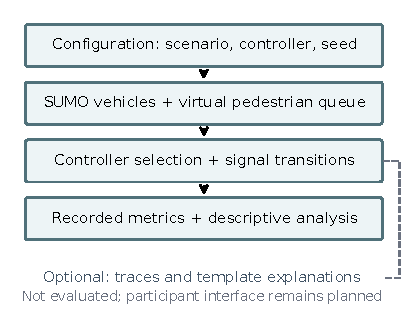
\includegraphics[width=\columnwidth]{figures/pipeline.pdf}
\caption{Implemented simulation workflow. The optional explanation path is shown separately because the matrix results evaluate allocation; they do not establish the quality of explanations or a participant-facing interface.}
\label{fig:pipeline}
\Description{Configuration feeds a SUMO and virtual-queue model, then controller selection and signal execution, then recorded metrics. An optional branch exports traces and template explanations.}
\end{figure}

Pedestrians are not SUMO walking agents in these runs. At each
one-second step, a seeded Bernoulli draw can add one pedestrian to
the virtual queue. During the pedestrian-service interval, at most
one queued pedestrian is removed per second. Vehicle demand is
generated from the bundled route flows and rescaled to the configured
rate. Thus, nominal inputs are paired across controllers, while actual
vehicle insertion can depend on congestion.

The separation in Figure~\ref{fig:pipeline} defines the scope of the
evidence. Vehicle movement belongs to the microscopic simulator,
while pedestrian service belongs to the queue abstraction. The
controller sees a combined state, but this does not make both modes
equally detailed. Consequently, the experiment can compare how
service opportunities are allocated; it cannot determine whether a
particular pedestrian would finish crossing before the next vehicle
phase.

\subsection{Functional Design and Features}
The implemented controller enumerates one candidate for each of the
three target phases, using a configured service duration. For mode
$m\in\{p,v\}$, the service utility is
\begin{equation}
u_m(a)=\min\left(1,\frac{S_m(a)}{\max(1,q_m+\lambda_m H)}\right),
\end{equation}
where $S_m(a)$ is predicted service, $q_m$ is the current queue,
$\lambda_m$ is nominal arrival rate, and $H$ is the prediction
horizon. This quantity expresses a service fraction; it is not a
measure of a person's satisfaction.

The denominator includes both the current queue and expected
arrivals within the horizon. This allows the controller to compare
predicted service against anticipated demand rather than the queue
alone. The upper bound of one prevents additional predicted service
from increasing utility after that demand estimate is covered.
Utility is therefore a normalized planning quantity, not an observed
outcome or a direct interpersonal comparison.

EFPB increases the weight of a mode as its longest wait approaches
its configured limit:
\begin{align}
\widetilde{\omega}_m&=\pi_m
\left[1+\kappa\min(1,W_m/T_m)^\eta\right],\\
\omega_m&=\frac{\widetilde{\omega}_m}
{\widetilde{\omega}_p+\widetilde{\omega}_v}.
\end{align}
The frozen SUMO settings use equal base weights, $\kappa=2$,
$\eta=1$, $H=60$~s, a 25~s candidate duration, and
$T_p=T_v=100$~s. The controller is reconsidered every second, subject
to execution timing; the candidate duration is therefore a planning
quantity rather than an assurance that the phase remains active for
exactly 25~s.

The weight rule expresses urgency through the longest recorded
wait. Because the waiting ratio is capped at one inside this rule,
the weight stops increasing once the configured limit is reached.
The separate feasibility check and fallback are therefore important:
the weight formula alone cannot guarantee service under persistent
overload. This is also why we retain both average waiting and
maximum-wait measures in the evaluation.

The predicted loss combines queue-based delay estimates and a
switch penalty. After the applicable feasibility checks, EFPB keeps
plans satisfying
\begin{equation}
L(a)\leq L_{\min}+\delta\max(L_{\min},L_{\mathrm{floor}}),
\end{equation}
with $\delta=0.05$ and $L_{\mathrm{floor}}=1$. It then maximizes
the weighted log bargaining score
\begin{equation}
B(a)=\sum_{m\in\{p,v\}}\omega_m
\log\!\left(\max\{\epsilon,u_m(a)-d_m+\epsilon\}\right),
\end{equation}
where $\epsilon=10^{-6}$ and $d_m$ is the utility of holding the
current phase in this implementation. If the individually rational,
predicted-wait-feasible set is empty, EFPB uses a least-breach
fallback. Consequently, the 100~s limit is not an unconditional
guarantee, and the efficiency tolerance constrains predicted loss
within the retained set, not measured trip delay.

The baselines share the state representation and signal execution.
Fixed time uses a calibrated 37~s cycle. Its plan generator is
demand-based, but at the selected minimum cycle all available time
is consumed by minimum greens and transition allowances, leaving
no surplus to redistribute by demand. Efficiency-only control
minimizes predicted loss. Equal bargaining uses equal mode weights
without EFPB's waiting-weight and near-efficiency mechanisms.
These differences make the comparison interpretable, while the
equal-bargaining feasibility behavior requires special caution.

The baselines answer different comparison questions. Fixed time
provides a regular service schedule; efficiency-only control isolates
the predicted-loss objective; equal bargaining retains a bargaining
objective without EFPB's additional waiting and efficiency rules.
They should not be interpreted as three interchangeable measures of
existing practice. In particular, the internal bargaining baseline is
useful for examining this implementation, but is not a substitute for
a carefully reproduced prior controller.

\subsection{Interface Design and Interaction Flow}
The current interaction is an experiment-review workflow. A
researcher selects a configuration and controller, starts a run,
checks its completion record, and compares the resulting metrics
with runs using the same scenario and seed. Stored identifiers and
configuration fingerprints connect a result to its experimental
conditions.

For public or operator use, the proposed interaction would be to
view the decision, inspect its reason, compare an alternative, and
review the history. A decision card would pair the phase name with
plain language and visible units. An alternative panel would report
the search limits as well as a successful decision flip. This is a
design specification, not a description of screens used by study
participants.

For example, an operator investigating a long wait would first need
the timestamp and actual signal state, then the waiting values used
at that decision, and finally the feasible alternatives. Presenting
these in the reverse order would require the operator to interpret a
score without knowing what happened. This proposed sequence also
gives missing data a visible place: an unavailable trace should be
shown as unavailable, rather than replaced with a plausible reason.

\subsection{Human-Centered AI Implementation}
AI in this project takes the form of explicit decision rules and
optimization, rather than a trained predictor or generative language
model. The intended benefit is inspectability: service estimates,
weights, and restrictions can be examined directly.

The software defines a \texttt{DecisionTrace} with the observed
state, selected candidate, weights, reason facts, a rejected-candidate
identifier, and configuration and trace hashes. Template functions
can turn recorded values into factual text. A bounded search changes
selected input features and replays the controller to look for a
decision flip. This does not establish a globally nearest feasible
counterfactual. Nor does a populated reason field prove that a
constraint caused the action. Those stronger properties require
targeted fidelity checks and execution-aligned traces.

Three levels of explanation must remain distinct. A factual account
reports the recorded choice and its inputs. A contrastive account
compares that choice with a named alternative. A counterfactual
account changes an allowed input and checks whether replay changes
the choice. The last two require more than a well-formed sentence:
they need the relevant candidate information or replay result.
Their evaluation cannot be inferred from the traffic metrics.

\subsection{Implementation Details}
The experiment reports document several corrections that materially
affected the results: selecting the intended SUMO signal program,
matching approach groups to phases, scaling vehicle demand,
adding yellow/all-red transitions, and preventing parallel clients
from connecting to the wrong simulation~\cite{runreport}. Earlier
invalid pilots and stale surrogate results were excluded from the
evidence used here.

The analyzed SUMO runner is version 0.5.0. Vehicle transitions use
3~s yellow and, between vehicle groups, 1~s all-red; minimum green
is 10~s. These timings do not implement a physical pedestrian
clearance model. Other departures from the full methodology include
single-phase candidates rather than multi-phase plan sequences,
queue-based rather than total-delay max-pressure direction logic,
and missing emergency, sensor-error, and accessibility handling in
the SUMO matrix. These are limits of the evaluated implementation,
not features established by the results.

\section{Evaluation}
\subsection{Experimental Design}
The completed evaluation is a simulation study with no human
participants. Its main factorial design contains 13 demand cells,
four controllers, and ten paired random seeds, giving 520 runs.
Nine nominal cells combine pedestrian and vehicle demand levels
L, M, and H. Four stress cells use S/S, H/S, S/H, and O/O, where
S and O denote near-saturation and overload settings
(Table~\ref{tab:demand}). Every run lasts 4,200 simulated seconds:
600~s warm-up and 3,600~s evaluation. Seeds 4001--4010 are shared
across controllers and are disjoint from calibration and pilot seeds.

\begin{table}[!htbp]
\caption{Nominal arrival settings. Vehicle values are target aggregate rates; realized insertion may be lower under congestion.}
\label{tab:demand}
\small
\begin{tabular*}{\columnwidth}{@{\extracolsep{\fill}}lrr@{}}
\toprule
Level & Pedestrians/s & Vehicles/s\\
\midrule
L & 0.030 & 0.10\\
M & 0.070 & 0.22\\
H & 0.110 & 0.34\\
S & 0.225 & 0.66\\
O & 0.300 & 0.88\\
\bottomrule
\end{tabular*}
\end{table}

Controller and demand cell are the independent variables. Recorded
delay, maximum-wait ratio, mode-specific waiting, and simulator
event counts are the dependent variables. This design tests
allocation behavior under repeatable demand settings; it cannot
test usability or perceived fairness.

The demand grid is intended to reveal interactions between the two
modes, not simply to increase traffic in both at once. A condition
with high pedestrian demand and low vehicle demand asks a
different allocation question from its reverse. The mixed stress
cells serve the same purpose near capacity. These settings are
controlled synthetic conditions, not estimates of how often those
traffic patterns occur at a real intersection.

The accompanying results document identifies these runs as
exploratory because prior external registration of the protocol was
not established~\cite{resultsreport}. We preserve that status even
where configuration names contain the word \emph{confirmatory}.
A separate 36-run SUMO pilot and calibration sweeps provide
development context. They are not added to the 520-run sample.

\subsection{Procedure}
Calibration first explored demand levels and controller settings.
Each controller had a ceiling of 30 candidate configurations:
14 were evaluated for fixed time, 27 for efficiency, nine for equal
bargaining, and 30 for EFPB. Selection used seeds 301--305 and
scaled delay and maximum-wait objectives within each controller.
The selected settings were then compared with defaults on fresh
SUMO seeds 361--370. The final SUMO configuration retained the
default adaptive-controller settings and the 37~s fixed-time plan.
Calibration observations were not treated as independent evaluation
results.

The matrix then crossed each demand cell with every controller and
seed. Runs used the same configured input rates and seed within
each matched comparison. The supplied reports describe execution
on an Ubuntu laptop with an AMD Ryzen 7 5800U, eight cores,
16 threads, and approximately 30~GB RAM.

For this report, we inspected the configuration and analysis code
and independently recomputed the cell means, group means, and
paired differences from the 520 supplied per-run CSV rows.
All 52 controller--cell combinations contained ten unique seeds.
The recomputed summaries agreed with the supplied tables within
numerical precision. This checks the arithmetic and completeness
of the result tables; it is not a rerun of SUMO. Raw trajectory
files and individual run metadata were not included in the shared
evidence.

Pairing is important because a random arrival realization can affect
the observed waits. Comparing controllers within the same
scenario--seed combination provides a more interpretable contrast
than comparing unrelated runs. It does not make the resulting
trajectories identical: controller decisions change queues, and
congestion can change vehicle insertion. The shared seed is a
design control, not a guarantee that every recorded road-user
population is the same.

\subsection{Evaluation Metrics}
The principal efficiency measure is the repository's recorded
person-delay proxy. For the recorded pedestrian and vehicle
populations, it combines pedestrian waiting with vehicle stopped
time using assumed occupancy $o=1.3$:
\begin{equation}
\widehat D=
\frac{N_p\overline W_p+oN_v\overline S_v}
     {N_p+oN_v}.
\label{eq:delay}
\end{equation}
Here $\overline S_v$ is stopped time, not full travel-time loss
relative to free flow. Counts include recorded completions and
specified unfinished records. This distinction matters when
congestion prevents vehicles from entering the network.

The waiting safeguard is summarized as
\begin{equation}
\mw=\max\!\left(\frac{W_p^{\max}}{100},
                 \frac{W_v^{\max}}{100}\right).
\end{equation}
Values above one indicate that the recorded maximum exceeded
the configured limit. The vehicle component uses consecutive
stopped waiting samples, whereas pedestrian waiting is time in
the virtual queue. They are operational indicators of different
processes, not interchangeable measures of lived experience.

Equation~\ref{eq:delay} combines the recorded mode populations
within a run. The group summaries then average run and cell
metrics; they are not reconstructed by pooling all people from
every simulation. This distinction helps explain why a group-level
person-delay value cannot be recovered simply by averaging the
two mode-specific means in the results table. Their relative
contributions depend on the recorded counts as well as occupancy.

Pedestrian mean waiting, vehicle mean stopped time, and
simulator-reported collisions and emergency stops provide
additional context. No rationale-comprehension score, task
completion time, usability score, trust rating, interview theme,
or perceived-fairness measure is available.

\subsection{Analysis Approach}
We report means within each controller--cell combination and
then give equal weight to cells within nominal or stress groups.
Keeping those groups separate prevents overload behavior from
being hidden in a single overall average. For comparisons, the
difference is EFPB minus the baseline for the same scenario and
seed.

Table~\ref{tab:paired} reproduces descriptive mean differences
and standard errors calculated as the sample standard deviation
of paired differences divided by $\sqrt{n}$. These errors pool
cell--seed pairs and do not account for the shared seed structure
or strong differences between demand cells. They are not
cluster-adjusted uncertainty estimates. No significance tests,
preregistered mixed models, or causal attribution to an individual
EFPB component are claimed.

We use the paired table to describe the direction and size of the
observed differences. We do not read a small pooled standard error
as evidence that an effect will generalize to another junction or
demand process. Cell-level plots provide a complementary check:
they show whether a group average represents a recurring pattern
or conceals sharply different operating conditions.

\section{Results}
\subsection{Quantitative Results}
Table~\ref{tab:main} reports the main SUMO summaries. Across
nine nominal cells, EFPB's recorded person-delay proxy was
6.31~s, compared with 6.45~s for efficiency, 6.68~s for equal
bargaining, and 8.49~s for fixed time. The descriptive reduction
relative to fixed time is 2.18~s, or approximately 25.6\% of its
mean. The reduction relative to efficiency is much smaller:
0.13~s, approximately 2.1\%.

The table should be read across metrics as well as down controllers.
The delay column summarizes the recorded population-weighted
proxy; the other columns expose aspects that this average can
hide. A controller with a favorable delay value may still have a
larger longest wait or shift waiting from one mode to another.
The nominal and stress rows are therefore kept separate rather
than reduced to one overall ranking.

\begin{table}[!htbp]
\caption{Main SUMO results, averaged equally over nine nominal or four stress cells. Each controller--cell mean uses ten seeds. Delay is the recorded proxy in Equation~\ref{eq:delay}; vehicle stopping and virtual pedestrian waiting are distinct quantities.}
\label{tab:main}
\small
\setlength{\tabcolsep}{3pt}
\renewcommand{\arraystretch}{1.12}
\begin{tabular*}{\columnwidth}{@{\extracolsep{\fill}}lrrrr@{}}
\toprule
Controller & \shortstack{Delay\\(s)} & \shortstack{Max-wait\\ratio} & \shortstack{Ped. wait\\(s)} & \shortstack{Veh. stop\\(s)}\\
\midrule
\multicolumn{5}{@{}l}{\emph{Nominal demand: nine cells}}\\
Fixed time & 8.49 & 0.270 & 11.17 & 7.68\\
Efficiency & 6.45 & 0.467 & 8.68 & 6.20\\
Equal bargaining & 6.68 & 0.419 & 5.98 & 6.83\\
EFPB & 6.31 & 0.414 & 8.75 & 5.98\\
\midrule
\multicolumn{5}{@{}l}{\emph{Stress demand: four cells}}\\
Fixed time & 48.59 & 1.484 & 72.26 & 37.56\\
Efficiency & 41.06 & 1.855 & 34.64 & 129.11\\
Equal bargaining & 338.88 & 18.040 & 807.50 & 324.72\\
EFPB & 41.95 & 1.542 & 23.54 & 133.83\\
\bottomrule
\end{tabular*}
\end{table}

EFPB recorded a lower nominal mean delay than each comparator
in all nine cells. Maximum waiting shows a different pattern.
Fixed time had a mean maximum-wait ratio of 0.270, below EFPB's
0.414. EFPB was below efficiency's 0.467 in every nominal cell,
but was close to equal bargaining on this measure. Figure~\ref{fig:nominal}
shows why a single ranking would be incomplete.

Across the nominal cells, the delay difference between EFPB and
efficiency-only control remains visually small. The clearer
separation is between their maximum-wait ratios and that of the
short-cycle fixed-time plan. This is a useful distinction for
interpretation: EFPB offers a different balance of the two measures,
not an improvement on every measure at once. The points summarize
ten seeds each and do not display within-cell variability.

\begin{figure}[H]
\centering
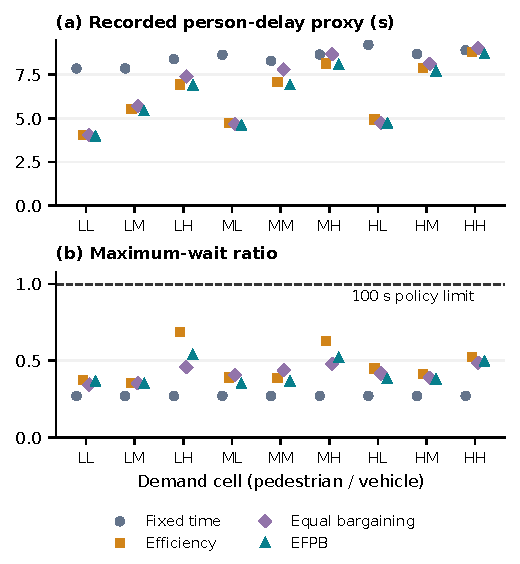
\includegraphics[width=\columnwidth]{figures/nominal_results.pdf}
\caption{Nominal SUMO results by demand cell; each point is the mean of ten runs. The first demand letter refers to pedestrians and the second to vehicles. The dashed line marks the 100~s policy threshold. No inferential error bars are shown.}
\label{fig:nominal}
\Description{Two stacked point plots compare delay and maximum-wait ratios across nine demand cells. EFPB has slightly lower recorded delay than efficiency; fixed time has the lowest maximum-wait ratio.}
\end{figure}

The nominal results show that lower aggregate delay does not
necessarily mean lower pedestrian waiting. Equal bargaining had
the lowest nominal pedestrian mean, 5.98~s, while EFPB averaged
8.75~s. Conversely, fixed time produced a higher average delay
but lower maximum-wait ratio. The relevant comparison therefore
depends on the stated service objective.

Under stress, efficiency and EFPB averaged 41.06~s and 41.95~s
on the delay proxy, respectively, while fixed time averaged
48.59~s. Equal bargaining rose to 338.88~s. In the overloaded
O/O cell, all controllers exceeded the waiting limit: mean
maximum-wait ratios were 4.448 for fixed time, 4.849 for
efficiency, 36.849 for equal bargaining, and 4.581 for EFPB.
Figure~\ref{fig:stress} separates these stress conditions.

The logarithmic axes in Figure~\ref{fig:stress} make the severe
equal-bargaining outcomes visible without compressing all other
controllers against the axis. Equal vertical distances represent
ratios, not equal differences in seconds. The plot therefore helps
locate the stressed conditions, while Table~\ref{tab:main} retains
the exact group-level values. Neither display should be read as
evidence that overload has been solved by EFPB.

\begin{figure}[H]
\centering
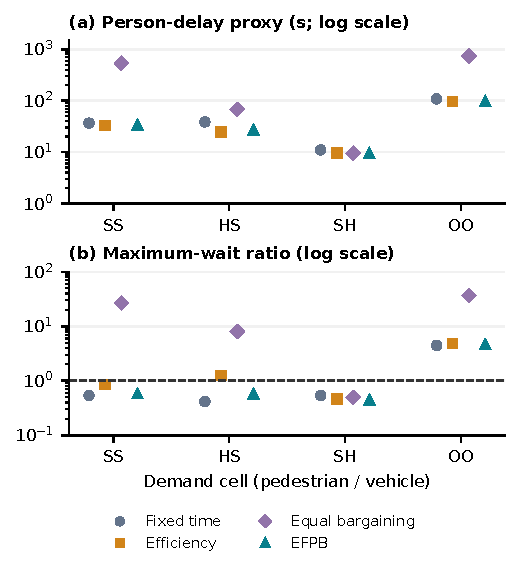
\includegraphics[width=\columnwidth]{figures/stress_results.pdf}
\caption{Stress-cell results, with logarithmic vertical axes to retain visibility of the large equal-bargaining values. Each point averages ten runs. In O/O, every controller's mean maximum-wait ratio exceeds one.}
\label{fig:stress}
\Description{Two stacked grouped point plots for SS, HS, SH, and OO show much larger delay and waits for equal bargaining under vehicle-heavy stress. All controllers exceed the wait threshold in OO.}
\end{figure}

All 520 SUMO result rows record zero collisions and zero emergency
stops. These counts concern the modeled vehicle simulation and
its evaluation window. They provide no direct evidence about
pedestrian trajectories or safety outside the model.

Zero recorded vehicle events and waiting-limit breaches describe
different outcomes. A run can avoid a collision while still delivering
poor service to a queue; a low average delay does not erase an
extreme wait.

\subsection{Qualitative Findings}
No participants supplied comments, and no observational usability
study was conducted. The qualitative material available consists
of engineering observations recorded during development.

One recurring issue was the difference between a controller's
intended action and its executed signal state. Incorrect phase
mapping initially caused the wrong states to be displayed.
Another was measurement bias: omitting unfinished queues made
starvation appear less severe. A third was baseline quality:
calibrating the fixed-time plan substantially changed the apparent
advantage of adaptive control~\cite{runreport}. These observations
explain implementation decisions, but they are not themes from
user interviews.

\subsection{Comparative Observations}
Table~\ref{tab:paired} makes the sign of each comparison explicit.
For nominal demand, EFPB's delay differences are negative against
all three baselines, but its maximum-wait difference is positive
against fixed time. Under stress, the large pooled errors indicate
substantial variation in the underlying paired differences. The
very large advantage over equal bargaining should be interpreted
alongside that comparator's documented feasible-set problem,
not as a general estimate of EFPB's advantage over bargaining.

\begin{table}[!htbp]
\caption{Descriptive paired comparisons: EFPB minus baseline, mean $\pm$ pooled standard error. Negative values mean a lower recorded metric for EFPB. There are 90 cell--seed pairs per nominal comparison and 40 per stress comparison; the errors are not adjusted for dependence across cells.}
\label{tab:paired}
\small
\setlength{\tabcolsep}{3pt}
\renewcommand{\arraystretch}{1.12}
\begin{tabular*}{\columnwidth}{@{\extracolsep{\fill}}lrr@{}}
\toprule
Baseline & \shortstack{Delay difference\\(s)} & \shortstack{Max-wait-ratio\\difference}\\
\midrule
\multicolumn{3}{@{}l}{\emph{Nominal demand: 90 matched pairs}}\\
Fixed time & $-2.178 \pm 0.164$ & $+0.144 \pm 0.009$\\
Efficiency & $-0.135 \pm 0.025$ & $-0.053 \pm 0.007$\\
Equal bargaining & $-0.363 \pm 0.041$ & $-0.005 \pm 0.008$\\
\midrule
\multicolumn{3}{@{}l}{\emph{Stress demand: 40 matched pairs}}\\
Fixed time & $-6.633 \pm 9.986$ & $+0.059 \pm 0.968$\\
Efficiency & $+0.898 \pm 13.913$ & $-0.313 \pm 1.417$\\
Equal bargaining & $-296.926 \pm 79.447$ & $-16.498 \pm 2.373$\\
\bottomrule
\end{tabular*}
\end{table}

The earlier 36-run pilot also illustrates why implementation checks
matter. With the old static fixed-time plan held constant for the
clearance comparison, adding signal clearance changed aggregate
emergency-stop counts from 79 to zero. Tuning the fixed-time plan
subsequently changed its mean vehicle stopped time from about
16.5~s to 8.1~s~\cite{resultsreport}. These are separate
development comparisons, not additional independent observations
for the main matrix.

The companion surrogate matrix contained 1,920 runs, of which
1,880 were analyzed after excluding the broken accessibility
condition. It is retained as engineering evidence only. The
different magnitudes and stress rankings across backends caution
against substituting surrogate numbers for SUMO observations.

\subsection{Summary of Key Findings}
EFPB recorded a small nominal-delay advantage over efficiency-only
control and a larger advantage over the calibrated fixed-time plan.
The fixed-time plan retained the strongest nominal maximum-wait
performance. Stress conditions exposed the limits of all four
controllers, especially the implemented equal-weight bargaining
baseline. The simulation recorded no vehicle collisions or emergency
stops in the main matrix. None of these findings establishes an
improvement in explanation understanding, usability, or trust.

\section{Discussion}
The nominal results suggest that waiting-sensitive allocation can
coexist with competitive average delay. That observation is
encouraging, but its size matters: the difference from efficiency-only
control is roughly a tenth of a second on the aggregate proxy.
There is no basis here for describing EFPB as a major efficiency
breakthrough.

Fixed time offers an important counterpoint. A short recurring
cycle gives each mode a predictable service opportunity. This
helps explain its lower maximum-wait ratio even when its mean
delay is higher. From an HCI perspective, predictability may be
valuable to a person waiting at a crossing, but the present study
did not measure that value. An interface should make this
trade-off visible instead of describing one policy simply as
fairer.

Equal mode weights, low average delay, and bounded waiting encode
different priorities. An operational policy would need to state and
justify its choice. The side-by-side metrics make that trade-off
inspectable without deciding which policy a community should prefer.

The stress results expose a structural weakness in the internal
equal-bargaining baseline. Its disagreement point is the current
phase. If a switch reduces vehicle utility while a vehicle queue
remains, the individual-rationality rule can reject that switch,
leaving pedestrians without service. Large EFPB advantages over
this comparator therefore reflect, at least in part, a weakness in
the comparator's implemented feasible set. They cannot establish
superiority over published bargaining methods.

There is also a limit to what can be attributed to EFPB's Nash
score. Its least-breach rule can reduce selection to a single
candidate before bargaining occurs. Without working ablations,
we cannot determine how much of the observed behavior comes
from waiting-based weights, efficiency filtering, or that fallback.
The weak response to the calibration sweep over $\delta$ is
consistent with this concern, but does not prove its cause.

Finally, the development history connects explanation fidelity to
execution fidelity. A clear explanation of a requested phase can
still mislead if the signal displays a different phase or delays the
change for clearance. A useful audit interface must distinguish
request, pending transition, and actual execution. It must also
show a failure or fallback plainly; polished text should not turn
a capacity shortage into a claim that everyone was treated well.

Fluent explanations could otherwise make a weak controller seem
more credible. A later HCI study should ask whether readers can
identify an unsatisfactory decision and explain its limitation,
rather than merely repeat the controller's stated reason.

\section{Implications for Design}
First, show the allocation trade-off in terms people can compare.
Average delay, longest wait, and mode-specific waiting should be
visible together. The results demonstrate why a single green
fairness indicator would hide relevant information.

A compact summary could show the selected mode, both modes'
current waits, and the labeled policy target. Historical averages
could remain available for review, but should not be used to
justify every individual choice.

Second, design the explanation around a decision record that is
linked to execution. A user should be able to inspect what was
requested, what was displayed, and whether a transition or
override intervened. Values and units should come from that
record, with an explicit message when evidence is unavailable.

Third, describe limits honestly. A 100~s policy target is not a
promise when demand exceeds capacity. A counterfactual search
that finds no flip should disclose its tested range, rather than
imply that no alternative is possible.

A capacity-related fallback concerns the available service choices;
a failed counterfactual search concerns the tested alternatives.
These need distinct messages so that an operator knows what to
investigate, even without opening the mathematical details.

Fourth, give users different depths of explanation. A brief
statement may be enough to orient a pedestrian reviewing a
decision; an operator may need the candidate comparison and
history. These are design recommendations that still require
user evaluation.

Finally, evaluate whether explanations help people reject an
inappropriate decision as well as recognize an appropriate one.
A follow-up study should compare decision-only, factual, and
factual-plus-counterfactual conditions using matched replays,
objective rationale and decision-flip questions, response time,
and appropriately interpreted fairness and trust measures.
The relevant success criterion is informed judgment.

Such a study should keep the underlying decisions matched across
explanation conditions, so that an easier scenario is not mistaken
for a better explanation. It should also include decisions with
visible limitations, rather than only successful nominal cases.
Any improvement in confidence would then need to be considered
alongside accuracy and response time. These are proposed study
controls, not procedures completed in the present project.

\section{Limitations}
The most direct limitation is the absence of a participant study.
There are no completed interviews, validated personas, usability
sessions, or human trust and fairness measurements. The HCI
contribution at this stage consists of a reasoned design and an
evaluation plan, supported by technical observations.

The SUMO model also has a limited scope. It covers one junction,
with virtual pedestrian service and synthetic demand. Walking
trajectories, crossing duration, mobility differences, and pedestrian
clearance are not modeled. Emergency, sensor-error, bursty-demand,
and accessibility fields are not exercised by the SUMO matrix.
Zero recorded vehicle events cannot establish real-world or
pedestrian safety.

The single-junction setting also excludes coordination with
neighboring signals and downstream space constraints. Those
conditions require further modeling; the same controller ordering
cannot be assumed to persist across a network.

The metrics require particular care. Although the execution report
describes a post-warm-up arrival cohort, inspection of runner 0.5.0
shows that completions after warm-up can retain waiting accumulated
earlier. Its unfinished-vehicle count is based on vehicles with
recorded stopped steps, not every vehicle still present. Vehicles
delayed before insertion are outside the measured population.
The saved summaries therefore support the reported proxies, not
a verified measure of total person delay for all intended arrivals.
This is especially consequential under overload. Raw trajectories
and individual metadata would be needed to quantify the effects
and reconstruct stricter metrics.

The matrix uses ten seeds per cell, fewer than the original
30-seed plan. Its analyses are exploratory, descriptive, and based
on fixed selected conditions. Pooled standard errors do not handle
all dependencies. Frozen settings reduce tuning on the evaluation
seeds, but do not turn the experiment into a preregistered study.
Calibration disclosures include discarded defective selections and
a tie-rule refinement made after inspection.

Finally, the implementation does not fully realize the original
controller and explanation specification. Multi-phase candidate
plans, total-delay max-pressure allocation, complete ablations,
globally nearest feasible counterfactuals, and independently
validated binding-constraint explanations remain outstanding.
The published per-run result tables were sufficient to check
summary arithmetic, but not to verify all trajectory-level behavior.

\section{Conclusion}
This project developed an explanation-oriented pedestrian--vehicle
priority prototype and evaluated its implemented controller in
520 exploratory SUMO/TraCI runs. The results show a useful but
qualified pattern: EFPB recorded low average delay under nominal
demand, while a calibrated short-cycle fixed-time controller kept
maximum waits lower. Overload exposed limits in every controller
and severe starvation in the internal equal-bargaining baseline.

The main lesson is that a credible human-centered traffic system
needs more than an attractive allocation score. Its decisions,
execution, and measurements must agree, and its explanations must
make the resulting trade-offs understandable. The next stage
should correct and validate the remaining measurement and
pedestrian-model limitations, implement meaningful ablations,
and evaluate the explanation interface with participants. The
current evidence supports that next stage; it does not yet
establish improved human understanding, calibrated trust, or
real-world fairness.

\bibliographystyle{ACM-Reference-Format}
\bibliography{references}
\end{document}
